%LTeX: language=it
\chapter{03-03-2020, 05-05-2020}
\section{Scattering Rutherford}
\subsection{Calcolo della sezione d'urto}
Definendo le seguenti quantità:
\begin{itemize}
	\item $\phi$: flusso di particelle $\alpha$ incidenti sul campione
	\item $N_{\text{eventi}}$: il numero di eventi di scattering
	\item $N_{\text{target}}$: il numero di atomi target sul campione
	\item $\sigma$: la \textbf{sezione d'urto} del processo considerato
\end{itemize}
A seguito di alcune considerazioni\footnote{Approfondire questo aspetto}
possiamo ottenere la seguente relazione:
\begin{equation}
	\boxed{\mdv{N_{\text{eventi}}}{t} = \phi N_{\text{target}} \sigma}
\end{equation}
Per analisi dimensionale $\sigma$ dovrà avere le dimensioni di una superficie,
quindi $\msb{\sigma} = l^2$.\par Con una \textit{visione classica} potremmo
associare quella che abbiamo definito come sezione d'urto alla superficie utile
per ogni particella $\alpha$ del flusso incidente affinché il processo di
scattering \textbf{possa} (\textit{quindi stiamo implicitamente definendo il
	processo come probabilistico}) avvenire.

\paragraph{$\boldsymbol{\sigma\mrb{\theta\ge\tilde\theta}}$}
Ci interessa ora calcolare la \textbf{sezione d'urto} necessaria affinché il
processo di scattering causi una deflessione di un angolo
$\theta\ge\tilde\theta$, dove $\tilde\theta$ è un angolo di
riferimento\footnote{
	Ricorda l'angolo di deflessione è legato al parametro d'impatto tramite
	l'equazione \ref{eq:impact_parameter_angle}
}.
\begin{equation}
	\sigma\mrb{\theta\ge\tilde\theta} = \pi b^2\mrb{\theta=\tilde\theta}
	= \frac{\pi\rho^2}{\msb{2\tan{\frac{\tilde\theta}{2}}}^2} =
	\pi\msb{\frac{zZe^2}{4\pi\epsilon_0K}}^2
	\frac{1}{4}\cot^2{\frac{\tilde\theta}{2}}
\end{equation}
Volendo esprimere $\sigma$ in termini della \textit{costante di struttura
	fine}\footnote{
	Ricorda $\alpha= \frac{e^2}{4\pi\epsilon_0 \hbar c} \simeq \frac{1}{137}$
} abbiamo:
\begin{equation}
	\sigma\mrb{\theta\ge\tilde\theta} =
	\frac{\pi}{4}\msb{\frac{zZe^2}{4\pi\epsilon_0} \, \frac{\hbar c}{\hbar
			c}}^2 \frac{1}{K^2}\cot^2{\frac{\tilde\theta}{2}} = \frac{\pi}{4}
	\mrb{zZ}^2\alpha\mrb{\frac{\hbar c}{K}}^2\cot^2{\frac{\tilde\theta}{2}}
\end{equation}

\subsection{Sezione d'urto differenziale}
Poiché $\sigma = \pi b^2$, derivando rispetto a b e separando le quantità
infinitesime abbiamo:
\begin{equation}
	\mdv{\sigma}{b} = \mdv{}{b}\mrb{\pi b^2} = 2\pi b
\end{equation}
Quindi:
\begin{equation}
	\boxed{\md{\sigma} = 2\pi b \md{b}}
	\label{eq:sez_urto_diff_b}
\end{equation}
Ma conoscere la sezione d'urto differenziale espressa in funzione del parametro
d'urto $b$ è poco utile,
quindi tentiamo un \textbf{cambio di variabili} per riportare la
\textit{sezione d'urto differenziale in funzione
	dell'angolo di deflessione} $\theta$.
Sappiamo che:
\begin{equation}
	\mdv{b}{\theta} =
	\mdv{}{\theta} \mrb{\frac{\rho}{2\tan\frac{\theta}{2}}} =
	-\frac{\rho}{2\tan^2\frac{\theta}{2}} \,
	\mdv{}{\theta} \mrb{\tan\frac{\theta}{2}} =
	-\frac{\rho}{2\tan^2\frac{\theta}{2}} \,
	\frac{1}{2}\sec^2{\frac{\theta}{2}}
\end{equation}
Quindi abbiamo ottenuto la seguente relazione differenziale fre il parametro
d'impatto e l'angolo di deflessione:
\begin{equation}
	\md{b} = -\frac{\rho}{4\sin^2{\frac{\theta}{2}}} \, \md{\theta}
\end{equation}
Quindi possiamo concludere, sostituendo all'interno dell'equazione
\ref{eq:sez_urto_diff_b}:
\begin{equation}
	\md{\sigma} = 2\pi b = 2\pi\frac{\rho}{2\tan\frac{\theta}{2}} \md{b} =
	2\pi \frac{\rho}{2\tan\frac{\theta}{2}}
	\frac{\rho}{4\sin^2\frac{\theta}{2}} \md{\theta} =
	\frac{\rho^2 \cos\frac{\theta}{2}
		\sin\frac{\theta}{2}}{8\sin^4\frac{\theta}{2}}2\pi \md{\theta}
\end{equation}
Ora tramite le formule di bisezione per seno e coseno possiamo riscrivere il
numeratore come:
\begin{equation}
	\cos\frac{\theta}{2}\sin\frac{\theta}{2} = \frac{\sin\theta}{2}
\end{equation}
e sostituendo in $\md{\sigma}$ otteminamo:
\begin{equation}
	\md{\sigma} = \frac{\rho^2}{16\sin^4 \frac{\theta}{2}} 2\pi\sin\theta \,
	\md{\theta}
\end{equation}
Osserviamo che $2\pi\sin\theta \, \md{\theta} = \md{\Omega}$ è l'\textbf{angolo
	solido di deflessione} infinitesimo, quindi:
\begin{equation}
	\md{\sigma} = \frac{\rho^2}{16\sin^4 \frac{\theta}{2}} \, \md{\Omega}
\end{equation}
Da cui scriviamo:
\begin{equation}
	\textbf{Sezione d'urto differenziale su angolo solido}
	\qquad
	\boxed{\frac{d\sigma}{d\Omega} = \frac{\rho^2}{16\sin^4 \frac{\theta}{2}}}
\end{equation}
Scrivendo $\rho$ in forma estesa (\ref{eq:dist_max_avvicinamento}) diventa:
\begin{equation}
	\frac{\md{\sigma}}{\md{\Omega}}
	= \frac{1}{16} \mrb{zZ}^2 \alpha^2 \mrb{\frac{\hbar c}{K}}^2
	\frac{1}{\sin^4\frac{\theta}{2}}
	= \frac{1}{16} \mrb{zZ}^2 \alpha^2 \msb{\frac{2m}{m^2v^2}}^2
	\frac{1}{\sin^4\frac{\theta}{2}}
	\label{eq:sez_urto_diff_alpha}
\end{equation}

\begin{note}[Divergenza della sezione d'urto]
	La sezione d'urto differenziale per scattering Rutherford, formulata
	considerando l'interazione coulombiana come unica forma d'interazione, in
	regime classico, e non considerando la carica del nucleo schermata dagli
	elettroni, presenta una divergenza per $\theta \to 0$.
\end{note}

\paragraph{Impulso trasferito}
L'impulso come grandezza vettoriale non è una quantità conservata, ma ne è
conservato il modulo,
ovvero $\abs{\vec{p}_f} = \abs{\vec{p}_i}$.

La quantità:
\begin{subequations}
	\begin{equation}
		\vec{q} = \vec{p}_f-\vec{p}_i = m \mrb{\vec{v}_f - \vec{v}_i}
		\label{eq:impulso_trasferito}
	\end{equation}
	\begin{equation}
		\abs{\vec{q}\,} = 2mv \, \sin\frac{\theta}{2}
		\label{eq:modulo_q}
	\end{equation}
\end{subequations}
mostrata in figura~\ref{fig:impulso_trasferito} è detta \textbf{impulso
	trasferito nel processo d'urto} e rappresenta la \textit{variazione di impulso
	della particella scatterata, che è l'impulso	assorbito dall'atomo
	scatterante}.

\begin{figure}[ht]
	\centering
	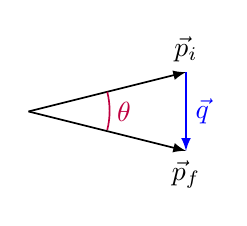
\begin{tikzpicture}
		\draw[semithick, -latex] (0,0) -- (2,0.5) node[above]{$\vec{p}_i$};
		\draw[semithick, -latex] (0,0) -- (2,-0.5) node[below]{$\vec{p}_f$};
		\draw[semithick, -latex, color=blue] (2,0.5) -- (2,-0.5);
		\draw[color=blue] (2,0) node[right]{$\vec{q}$};
		\draw[semithick, color=purple] (1,0.25) arc [radius=1, start angle=14.036, end angle=-14.036];
		\draw[color=purple] (1,0) node[right]{$\theta$};
	\end{tikzpicture}
	\caption{Impulso trasferito}
	\label{fig:impulso_trasferito}
\end{figure}

Con questa nuova definizione riprendiamo la sezione d'urto differenziale
dall'equzazione \ref{eq:sez_urto_diff_alpha} e sostuiamo l'equazione
\ref{eq:modulo_q} appena trovata:
\begin{align}
	\textbf{Sezione d'urto differenziale di Rutherford} &  &
	\boxed{
		\frac{\md{\sigma}}{\md{\Omega}} = 4\mrb{zZ}^2 \alpha^2 \mrb{\hbar c}^2
		\frac{m^2}{q^4}
	}
	\label{eq:sezione_urto_differenziale_rutherford}
\end{align}

\begin{note}[]
	Nell'ipotesi di atomo \textit{non rinculante} c'è solo trasferimento di
	impulso, ma non c'è trasferimento di energia.
\end{note}

\subsection{Calcolo Quantistico della sezione d'urto}
Il calcolo quantistico della sezione d'urto dello scattering Rutherford può
essere effettuato utilizzando la \textit{Regola d'oro di Fermi}, definita come
segue:
\begin{align}
	\textbf{Regola d'Oro di Fermi} \qquad
	\boxed{
		\md{\omega_{if}} = \frac{2\pi}{\hbar} \, \abs{T_{if}^\prime}^2 \,
		\delta\mrb{E_i-E_f} \md{n_f}
	}
	\label{eq:regola_oro_fermi}
\end{align}
Dove $\ket{i}$ e $\ket{f}$ sono rispettivamente gli stati \textit{iniziale} e
\textit{finale} del processo e $\hat{\ham} = \hat{\ham}_{0} +
	\hat{\ham}_{\text{int}}$ l'Hamiltoniana totale del sistema, definiamo le
seguenti grandezze:
\begin{itemize}
	\item $\md{\omega_{if}}$: probabilità di transizione per unità di tempo (le
	      dimensioni fisiche saranno $\msb{\si{\per \s}}$);
	\item $E_i,E_f$: energie degli stati iniziale e finale;
	\item $T_{if}^\prime$: elemento di matrice;
	      $\bra{f}\hat{\ham}_{\text{int}}\ket{i}$ dell'Hamiltoniana di interazione
	\item $\md{n_f}$: \# di stati finali accessibili per il sistema,
	      ovvero\footnote{
		      La grandezza $\rho\mrb{E_f}$ indica la densità di stati in funzione
		      dell'energia e $\md{E}_{f}$ l'intervallo infinitesimo di energia
	      } $\rho\mrb{E_f} \md{E_f}$;
	\item $\delta\mrb{E_f - E_i}$: delta di Dirac di \textbf{conservazione
		      dell'energia}.
\end{itemize}

\paragraph{Definire stati iniziale e finale}
Supponiamo stati iniziale e finale \textit{autostati dell'impulso} (stati ad
impulso definito):
\begin{subequations}
	\begin{equation}
		\ket{i} = \ket{\vec{p}_i}
	\end{equation}
	\begin{equation}
		\ket{f} = \ket{\vec{p}_f}
	\end{equation}
\end{subequations}
Inoltre sappiamo gli autostati dell'impulso essere rappresentati nella base
degli \textit{autostati della posizione} da \textbf{onde piane}, quindi abbiamo
la forma seguente:
\begin{subequations}
	\begin{equation}
		\braket{\vec{x}\vert\vec{p}_i} = A \exp{\mcb{i \,
				\frac{\vec{p}_i\cdot\vec{x}}{\hbar}}}
	\end{equation}
	\begin{equation}
		\braket{\vec{x}\vert\vec{p}_f} = A \exp{\mcb{i
				\,\frac{\vec{p}_f\cdot\vec{x}}{\hbar}}}
	\end{equation}
	\label{eq:coordinate}
\end{subequations}
dove $A$ rappresenta la \textit{costante di normalizzazione delle onde piane}.

Presentiamo ora una procedura tipica in fisica delle particelle: fissiamo la
normalizzazione della funzione d'onda introducendo un \textit{volume di
	normalizzazione}.

\paragraph{Volume di normalilzzazione}
La costante di normalizzazione può essere determinata in diversi modi. Uno di
questi è introdurre il \textbf{volume di normalizzazione} $V$, ovvero il volume
dello spazio tridimensionale all'interno del quale l'integrale del modulo
quadro della funzione d'onda sia uguale a 1. Facciamo questo per semplificare i
nostri calcoli, aspettandoci che il risultato finale sia indipendente dal
volume di normalizzazione utilizzato\footnote{
	Questo ci permette di determinare la normalizzazione degli stati, ma anche di
	calcolare il numero di stati finali accessibili dal sistema $\md{n_f}$,
	poiché questa è una grandezza che dipende da come normalizziamo i nostri
	stati
}. Quindi affinché gli stati
iniziale e finale siano normalizzati all'interno di tale volume di
normalizzazione, ovvero che:
\begin{equation}
	\braket{\vec{p}_{i,f} \vert \vec{p}_{i,f}} = 1 \rightarrow
	\mint{}{}{\vec{x}}{\abs{\braket{\vec{x} \vert \vec{p}_{i,f}}}^2} = 1
\end{equation}

Questo implica che il valore della costante $A$ nelle equazioni
\ref{eq:coordinate} sia $A = \frac{1}{\sqrt{V}}$, per cui:
\begin{subequations}
	\begin{equation}
		\braket{\vec{x}\vert\vec{p}_i} = \frac{1}{\sqrt{V}}\exp{\mcb{i \,
				\frac{\vec{p}_i\cdot\vec{x}}{\hbar}}}
	\end{equation}
	\begin{equation}
		\braket{\vec{x}\vert\vec{p}_f} = \frac{1}{\sqrt{V}}\exp{\mcb{i \,
				\frac{\vec{p}_f\cdot\vec{x}}{\hbar}}}
	\end{equation}
\end{subequations}

\begin{note}[]
	Dal punto di vista classico, una particella è identificata dalle $3$
	coordinate spaziali e dalle $3$ coordinate di impulso (\textit{spazio delle
		fasi classico}). Questo nel calcolo quantistico non vale, per cui diversi
	stati classici (nel limite del principio di indeterminazione) devono
	coincidere con un unico stato quantistico ($\Delta^3 x\, \Delta^3 p = h^3$).
	Quindi, avendo introdotto il \textit{volume di normalizzazione}, possiamo
	dire che $\Delta^3 x = V$, quindi:
	\begin{equation}
		\Delta^3 p = \frac{h^3}{V}
	\end{equation}
	La \textit{densità dei possibili stati}:
	\begin{subequations}
		\begin{equation}
			\mdv{n_f}{p} = \frac{V}{h^3}
		\end{equation}
		quindi in termini di $\hbar$:
		\begin{equation}
			\mdv{n_f}{p} = \frac{V}{\mrb{2 \pi}^{3} \hbar^3}
		\end{equation}
	\end{subequations}
\end{note}

A questo punto possiamo andare a calcolare l'elemento di matrice
$T_{if}^\prime$, ricordando che $\hat{\ham}_{\text{int}}$ è il
\textit{potenziale coulombiano} generato dal nucleo scatterante:
\begin{equation}
	T_{if}^\prime = \bra{f}\ham_{\text{int}}\ket{i} = \int \mathrm{d}^3\vec{x}
	\int \, \mathrm{d}^3\vec{y} \braket{f\vert\vec{x}\,}
	\bra{\vec{x}\,}\ham_{\text{int}} \ket{\vec{y}\,} \, \braket{\vec{y}\,\vert i}
	\label{eq:elemento_matrice_hamilt_interazione}
\end{equation}
poiché gli integrali sui proiettori $\ket{\vec{x}\,}\bra{\vec{x}\,}$ e
$\ket{\vec{y}\,}\bra{\vec{y}\,}$ sono proprio l'identità. Poiché possiamo
scrivere l'Hamiltoniana di interazione come (\textit{interazione
	coulombiana}\footnote{
	I potenziali di interazione che hanno andamento $\frac{1}{r}$ sono detti
	\textbf{potenziali a lungo raggio}
} dipendente solo dalla posizione),
scegliendo un sistema di riferimento in cui la particella che produce lo
scattering è posta nell'origine:
\begin{equation}
	\hat{\ham}_{\text{int}} = \frac{zZe^2}{4\pi\epsilon_0} \,
	\frac{1}{\abs{\vec{x}}\,}
	\label{eq:ham_int_puntiforme}
\end{equation}
dove chiaramente $z$ è la carica della particella scatterata e $Z$ la carica
del nucleo che produce l'effetto di scattering.
Quindi il termine $\bra{\vec{x}}\ham_{\text{int}}\ket{\vec{y}\,}$ farà
comparire una $\delta$ del tipo:
\begin{equation}
	\braket{\vec{x}\, \vert \hat{\ham} _{\text{int}} \vert \vec{y}\,} =
	\frac{zZe^2}{4\pi\epsilon_0} \, \frac{1}{\abs{\vec{x}}} \, \delta^{(3)}
	\mrb{\vec{x} - \vec{y}\,}
\end{equation}
La delta rimuoverà uno dei due integrali\footnote{Vedi proprietà della Delta di
	Dirac}, quindi continuiamo il calcolo dell'elemento di matrice riprendendo
dall'equazione \ref{eq:elemento_matrice_hamilt_interazione}:
\begin{equation}
	\begin{split}
		T_{if}^\prime & = \frac{1}{V} \int \mathrm{d}^3\vec{x} \, \exp{\mcb{-i \,
				\frac{\vec{p}_f\cdot\vec{x}}{\hbar}}} \,
		\hat{\ham}_{\text{int}}\mrb{\vec{x}\,} \, \exp{\mcb{i \,
				\frac{\vec{p}_i\cdot\vec{x}}{\hbar}}} \\
		& = \frac{1}{V} \int \mathrm{d}^3\vec{x} \,  \exp\mcb{-i \,
			\frac{\mrb{\vec{p}_f-\vec{p}_i}\cdot\vec{x}}{\hbar}} \,
		\hat{\ham}_{\text{int}}\mrb{\vec{x}\,} \\
		& = \frac{1}{V} \int \mathrm{d}^3\vec{x} \,  \exp\mcb{-i \,
			\frac{\mrb{\vec{p}_f-\vec{p}_i}\cdot\vec{x}}{\hbar}} \,
		\frac{zZe^2}{4\pi\epsilon_0} \, \frac{1}{\abs{\vec{x}}}
	\end{split}
\end{equation}
ed esprimendo in termini della quantità vettoriale \textit{impulso trasferito}
definita dall'equazione \ref{eq:impulso_trasferito}:
\begin{equation}
	T_{if}^\prime = \frac{1}{V} \int \mathrm{d}^3\vec{x} \, \exp\mcb{-i \,
		\frac{\vec{q}\cdot\vec{x}}{\hbar}} \, \frac{zZe^2}{4\pi\epsilon_0} \,
	\frac{1}{\abs{\vec{x}}}
	\label{eq:elemento_matrice_T_puntiforme}
\end{equation}
\textbf{Nota:} possiamo osservare che questa quantità, a meno della costante di
normalizzazione, è proporzionale alla \textit{\textbf{trasformata di Fourier}}
del potenziale di interazione con parametro della trasformazione definito
dall'impulso trasferito.
Questo ci dice che tanto maggiore è l'impulso trasferito, tanto più piccole
saranno le strutture che si possono osservare dei potenziali che mediano una
certa interazione (questo vale in generale, non solo per scattering
Rutherford).

Per calcolare l'integrale dato dall'equazione
\ref{eq:elemento_matrice_T_puntiforme} scegliamo un sistema di riferimento che
vede il vettore $\vec{q}$ diretto lungo l'asse $\hat{z}$ e il nucleo
scatterante posto nell'origine, come in figura:

\begin{figure}[ht]
	\centering
	\tdplotsetmaincoords{60}{110}
	\begin{tikzpicture}[scale=3,tdplot_main_coords]

		% variables
		\def\rvec{.8}
		\def\thetavec{30}
		\def\phivec{60}

		% axes & vector
		\coordinate (O) at (0,0,0);
		\draw[thick,-latex] (0,0,0) -- (1,0,0) node[anchor=north east]{$x$};
		\draw[thick,-latex] (0,0,0) -- (0,1,0) node[anchor=north west]{$y$};
		\draw[thick,-latex] (0,0,0) -- (0,0,1) node[anchor=south]{$z$};
		\draw[thick,-latex, color=blue] (0,0,0) -- (0,0,0.4) node[left]{$\vec{q}$};
		\tdplotsetcoord{P}{\rvec}{\thetavec}{\phivec}
		\draw[-latex,color=red, semithick] (O) -- (P) node[above right] {$\vec{r}$};

		% arcs
		\draw[dashed, color=red] (O) -- (Pxy);
		\draw[dashed, color=red] (P) -- (Pxy);
		\tdplotdrawarc{(O)}{0.2}{0}{\phivec}
		{anchor=north}{$\varphi$}
		\tdplotsetthetaplanecoords{\phivec}
		\tdplotdrawarc[tdplot_rotated_coords]{(0,0,0)}{0.5}{0}{\thetavec}
		{anchor=south west}{$\theta$}

	\end{tikzpicture}
	\caption{Scelta del sistema di riferimento}
	\label{fig:sistema_riferimento}
\end{figure}

Per cui l'equazione \ref{eq:elemento_matrice_T_puntiforme} diventa (dove
abbiamo utilizzato la notazione $r = \abs{\vec{x}}$ e $q = \abs{\vec{q}\,}$):
\begin{subequations}
	\begin{equation}
		\begin{split}
			T_{if}^\prime
			& = \frac{1}{V} \int_0^{2\pi} \! \mathrm{d}\varphi \int_{-1}^{1} \!
			\mathrm{d}\cos\theta \int_0^\infty \! \mathrm{d}r \,r^{\cancel2} \,
			\exp\mcb{i \, \frac{qr \cos\theta}{\hbar}} \frac{zZe^2}{4\pi\epsilon_0}
			\, \frac{1}{\cancel r}
			\\
			& = \frac{2 \pi}{V} \, \frac{zZe^2}{4\pi\varepsilon_0} \int_{-1}^{1} \!
			\mathrm{d}\cos\theta \int_0^\infty \! \mathrm{d}r \,r \exp\mcb{i \,
				\frac{qr \cos\theta}{\hbar}}
		\end{split}
		\label{eq:calcolo_elemento_matrice_T}
	\end{equation}
	per semplificare la notazione introduciamo la variabile $k = \frac {q}{r}$,
	per cui integrando prima in $\cos\theta$:
	\begin{equation}
		\begin{split}
			T_{if}^\prime
			& = \frac{2 \pi}{V} \, \frac{zZe^2}{4\pi\varepsilon_0} \int_0^\infty \!
			\mathrm{d}r \, \cancel r \frac{1}{ik \cancel r} \mcb{\exp\msb{ikr} -
				\exp\msb{-ikr}} \\
			& = \frac{2 \pi}{V} \, \frac{zZe^2}{4\pi\varepsilon_0} \,
			\frac{1}{\mrb{ik}^2} \mcb{\exp\msb{ikr}_0^\infty +
				\exp\msb{-ikr}_0^\infty}
		\end{split}
	\end{equation}
\end{subequations}
Ora, poiché $\exp\msb{ikr}$ ed $\exp\msb{-ikr}$ sono \textit{soluzioni
	oscillanti \textbf{non} dumpate}, l'integrale non converge. Abbiamo il problema
che non possiamo valutare esplicitamente l'integrale. Questo è legato al fatto
che il modello considerato è poco realistico, nel senso che il potenziale di
interazione considerato ha lo stesso comportamento in tutto lo spazio\footnote{
	Non viene considerata, ad esempio, l'azione schermante degli elettroni
	atomici degli atomi scatteranti. Infatti, a distanze minori della dimensioni
	caratteristiche dell'atomo l'interazione si sente; a distanze maggiori,
	invece, gli elettroni atomici schermano la carica del nucleo e l'interazione
	è dumpata
}. Nella realtà accade che ci sarà sempre una \textit{lunghezza di taglio}
oltre la quale il potenziale risulta schermato.

\paragraph{Taglio al potenziale di interazione} Ripetiamo ora il calcolo
dell'elemento introducendo un \textit{taglio (dump) esponenziale} al potenziale
di interazione coulombiano, che è un potenziale a corto raggio, per cui
riscriviamo l'Hamiltoniana di interazione come:
\begin{equation}
	\hat{\ham}_{\text{int}} = \frac{zZe^2}{4 \pi \varepsilon_0} \, \frac{1}{r}
	\exp\msb{-\mu r}
\end{equation}
dove $\mu$ può essere espresso in termini della lunghezza caratteristica $r_t$
chiamata \textbf{raggio di taglio}:
\begin{equation}
	\mu = \frac{1}{r_t}
\end{equation}
Si utilizza il taglio esponenziale poiché:
\begin{itemize}
	\item se $r \ll r_t$ l'Hamiltoniana di interazione descrive correttamente gli
	      effetti coulombiani
	\item se $r \gg r_t$ il termine esponenziale sopprime l'interazione
	      coulombiana
\end{itemize}
Torniamo al calcolo dell'integrale che descrive l'elemento di matrice
$T_{if}^\prime$, lasciato all'equazione \ref{eq:calcolo_elemento_matrice_T}
inserendo il termine aggiuntivo di taglio:
\begin{subequations}
	\begin{equation}
		\begin{split}
			T_{if}^\prime
			& = \frac{2\pi}{V} \, \frac{zZe^2}{4\pi\varepsilon_0} \int_{-1}^{1} \!
			\mathrm{d}\cos\theta \int_0^\infty \! \mathrm{d}r \, r e^{-\mu r}
			e^{ikr \cos\theta} \\
			& = \frac{2\pi}{V} \, \frac{zZe^2}{4\pi\varepsilon_0} \int_0^\infty \!
			\mathrm{d}r \, \frac{\cancel r}{ik \cancel r} e^{-\mu r} \,
			\mcb{e^{ikr} - e^{-ikr}} \\
			& = \frac{2\pi}{V} \, \frac{zZe^2}{4\pi\varepsilon_0} \int_0^\infty \!
			\mathrm{d}r \, \frac{1}{ik} \mcb{e^{-\mrb{\mu - ik}r} -
				e^{-\mrb{\mu + ik}r}} \\
			& = \frac{2\pi}{V} \, \frac{zZe^2}{4\pi\varepsilon_0} \, \frac{1}{ik}
			\mcb{\frac{1}{-\mrb{\mu - ik}} e^{-\mrb{\mu-ik}r}\Big\rvert_0^\infty -
				\frac{1}{-\mrb{\mu + ik}} e^{-\mrb{\mu+ik}r}\Big\rvert_0^\infty}
		\end{split}
	\end{equation}
	e poiché gli esponenziali, dumpati dall'introduzione di $\mu$, sono nulli se
	valutati all'infinito, l'espressione si riduce a:
	\begin{equation}
		\begin{split}
			T_{if}^\prime
			& = - \frac{2\pi}{V} \, \frac{zZe^2}{4\pi\varepsilon_0} \, \frac{1}{ik}
			\mcb{\frac{1}{-\mrb{\mu - ik}} - \frac{1}{-\mrb{\mu + ik}}} \\
			& = \frac{2\pi}{V} \, \frac{zZe^2}{4\pi\varepsilon_0} \, \frac{1}{ik}
			\mcb{\frac{\cancel\mu + ik - \cancel\mu + ik}{\mrb{\mu - ik}
					\mrb{\mu + ik}}} \\
			& = \frac{2\pi}{V} \, \frac{zZe^2}{4\pi\varepsilon_0} \, \frac{2}{\mu^2 +
				k^2}
		\end{split}
	\end{equation}
\end{subequations}
Quindi con il taglio esponenziale, e il parametro $\mu$, siamo in grado di
calcolare l'elemento di matrice:
\begin{equation}
	\textbf{Potenziale di Yukawa}\text{ ($r_t$ finita)}\qquad
	\boxed{
		T_{if}^\prime = \frac{4\pi}{V} \, \frac{zZe^2}{4\pi\varepsilon_0} \,
		\frac{1}{\mu^2 + k^2}
	}
\end{equation}
Nel caso \textit{coulombiano} mandiamo all'infinito la lunghezza di taglio
$r_t$ e otteniamo:
\begin{equation}
	T _{if} \mprime \xrightarrow{r_t \to \infty\ \Rightarrow\ \mu \to 0}
	\frac{4 \pi}{V} \frac{zZe^2}{4 \pi \eps_0} \frac{1}{k^2}
\end{equation}

Riprendendo la \textit{Regola d'oro di Fermi} (equazione
\ref{eq:regola_oro_fermi}), l'espressione che si ottiene quando
\textbf{rimuoviamo la lunghezza di taglio} $r_t$, ovvero quando $\mu \to 0$:
\begin{equation}
	\begin{split}
		\md{\omega_{if}}
		& = \frac{2\pi}{\hbar} \, \abs{T_{if}^\prime}^2 \, \delta\mrb{E_i - E_f}
		\, \md{n_f} \\
		& = \frac{2\pi}{\hbar} \, \mrb{\frac{4\pi}{V}}^2
		\mrb{\frac{zZe^2}{4\pi\varepsilon_0}}^2 \frac{1}{k^4} \,
		\delta\mrb{E_i - E_f} \, \md{n_f}
	\end{split}
	\label{eq:fermi_quasi_esplicita}
\end{equation}
Manipolando i termini per cercare un'espressione più compatta della formula,
con $\alpha$ la \textit{costante di struttura fine}:
\begin{equation}
	\frac{zZe^2}{4\pi\varepsilon_0} = \frac{zZe^2}{4\pi\varepsilon_0} \,
	\frac{\hbar c}{\hbar c} = zZ \alpha \hbar c
\end{equation}
in più, ricordando che $k = \nicefrac{q}{\hbar}$, ritroviamo un risultato già
ottenuto nel caso classico (equazione
\ref{eq:sezione_urto_differenziale_rutherford}) nella dipendenza da potenziale
coulombiano: in questo caso osserviamo che il tasso di transizione
$\md{\omega_{if}} \sim q^{-4}$.
Riscriviamo la \ref{eq:fermi_quasi_esplicita}, ricordando che $k =
	\frac{q}{\hbar}$:
\begin{equation}
	\md{\omega_{if}} = \frac{2\pi}{\hbar} \mrb{\frac{4\pi}{V}}^2 \mrb{zZ}^2
	\alpha^2 \mrb{\hbar c}^2 \frac{\hbar^4}{q^4} \, \delta\mrb{E_i - E_f}
	\md{n_f}
\end{equation}
\paragraph{Numero di stati finali accessibili dal sistema}
Ci rimane valutare il numero di stati finali accessibili dal sistema, ovvero la
\textit{conta degli stati} $\md{n_f}$.
Questo si può fare \textbf{imponendo le condizioni al bordo} oppure sfruttando
il \textbf{principio di corrispondenza}. Definiamo il \textbf{volume dello
	spazio delle fasi classico occupato da uno stato quantistico}: uno stato
quantistico, occupa nello spazio delle fasi classico, dato il \textit{principio
	di indeterminazione di Heisenberg}, un volume dato da:
\begin{equation}
	\boxed{\Delta^3p \, \Delta^3x = h^3}
\end{equation}
dove $\Delta^3x = V$ è proprio il \textit{volume di normalizzazione}, per cui
fissando lo spazio fisico in questo modo:
\begin{equation}
	\Delta^3p = \frac{h^3}{V}
\end{equation}
Per cui:
\begin{equation}
	\md{n_f} = \frac{\mathrm{d}^3p}{h}V
\end{equation}
Quindi possiamo dire che il numero degli stati finali accessibili dal sistema
ha una densità costante\footnote{
	La densità degli stati finali è \textit{uniforme} in $p$, poiché non c'è
	motivo che un impulso sia preferito rispetto ad un altro (\textit{isotropia})
} data da:
\begin{equation}
	\boxed{
		\frac{\md{n_f}}{\mathrm{d}^3p} = \frac{V}{h^3} = \frac{V}{\hbar^3
			\mrb{2\pi}^3}
	}
\end{equation}

\paragraph{Tasso di transizione}
In conclusione, mettendo insieme tutti i risultati ricavati fino ad ora,
possiamo dire che la \textit{probabilità di transizione per unità di tempo} per
il processo di \textit{scattering Rutherford} è data da:
\begin{equation}
	\md{\omega_{if}} = \frac{2\pi}{\cancel\hbar} \mrb{\frac{4\pi}{V}}^2 \alpha^2
	\mrb{\hbar c}^2 \frac{\cancel{\hbar^4}}{q^4} \mrb{zZ}^2
	\delta\mrb{E_i - E_f} \frac{V}{\cancel{\hbar^3} \mrb{2\pi}^3} \,
	\mathrm{d}^3p_f
	\label{eq:prob_transizione_unita_tempo}
\end{equation}
osserviamo che la quantità $\md{d}\omega_{if}$, ovvero la probabilità di
transizione per unità di tempo, conserva la dipendenza dal volume di
normalizzazione $V$. Questa quantità, però, non è l'osservabile fisico. Per
questo motivo andiamo a calcolare la sezione d'urto.

\paragraph{Sezione d'urto quantistica per Scattering Rutherford}
La sezione d'urto di questo processo è legata alla probabilità di transizione
per unità di tempo $d\omega_{if}$. La sezione d'urto ci dice quanto è probabile
che un processo di interazione fra ``\textit{proiettile}'' e
``\textit{bersaglio}'' avvenga.

In particolare, in questo caso abbiamo che il numero di eventi per unità di
tempo e per unità di tempo e unità di impulso dello stato finale:
\begin{equation}
	\frac{\md{N_\text{eventi}}}{\md{t} \, \mathrm{d}^3p_f} =
	\frac{\md{\sigma}}{\mathrm{d}^3p_f} \,
	\phi_p \,  N_t
\end{equation}
dove le quantità sono:
\begin{itemize}
	\item $\phi_p$ il \textit{flusso delle particelle (proiettili) incidenti};
	\item $N_t$ il \textit{numero di bersagli} illuminati dal fascio
	      (\textit{numero di target});
	\item $\frac{\md{\sigma}}{\mathrm{d}^3p_f}$ la \textit{sezione d'urto
		      differenziale} del processo definita in funzione dell'impulso della
	      particella nello stato finale.
\end{itemize}
Ricordiamo che nel nostro caso particolare si considera un singolo processo
(una particella su singolo bersaglio) all'interno di un volume di
normalizzazione, per cui, all'interno di quest'ultimo possiamo dire che:
\begin{equation}
	\begin{dcases}
		N_t = 1                     \\
		\phi_p = nv = \frac{1}{V} v \\
		\frac{\md{N_\text{eventi}}}{\md{t} \, \mathrm{d}^3p_f} =
		\frac{\md{\omega_{if}}}{\mathrm{d}^3p_f}
	\end{dcases}
\end{equation}
Dove per il flusso $\phi_p$: $v$ indica la \textit{velocità}
della particella $z$ incidente e $n$ indica la ``\textit{number density}'' di
particelle $z$ che collidono con il nucleo scatteratore e nel nostro caso
risulta essere $\nicefrac{v}{V}$ perché consideriamo una particella all'interno
del volume di normalizzazione.

Quindi possiamo scrivere che la sezione d'urto vale:
\begin{equation}
	\frac{\md{\sigma}}{\mathrm{d}^3p_f} = \frac{\md{N_\text{eventi}}}{\md{t} \,
		\mathrm{d}^3p_f} \, \frac{1}{\phi_\text{proiettili} N_t} =
	\frac{\md{\omega_{if}}}{\mathrm{d}^3p_f} \, \frac{V}{v}
\end{equation}
e sfruttando l'equazione \ref{eq:prob_transizione_unita_tempo}:
\begin{equation}
	\frac{\md{\sigma}}{\mathrm{d}^3p_f} = \msb{2\pi \mrb{\frac{4\pi}{\cancel
				V}}^2 \alpha^2 \mrb{\hbar c}^2 \frac{1}{q^4} \mrb{zZ}^2 \delta\mrb{E_i -
			E_f} \frac{\cancel V}{\mrb{2\pi}^3}} \frac{\cancel V}{v}
\end{equation}
quindi osserviamo che ora la sezione d'urto differenziale risulta del tutto
indipendente dal volume di normalizzazione $V$ e possiamo rielaborare e
semplificare ulteriormente ottenendo:
\begin{equation}
	\frac{\md{\sigma}}{\mathrm{d}^3p_f} = 4 \mrb{\hbar c}^2 \alpha^2 \mrb{zZ}^2
	\delta\mrb{E_i - E_f} \frac{1}{v} \, \frac{1}{q^4}
\end{equation}
In più, nel limite in cui il nucleo scatterante non rinculi, si avrebbe che
l'impulso finale $p_i$ coincide con l'impulso finale $p_f$ e si può descrivere
tutta la dinamica in termini dell'angolo solido $\Omega$, poiché potendo
scrivere:
\begin{equation}
	\mathrm{d}^3p_f = p_f^2 \md{p_f} \, \md{\Omega }
\end{equation}
dove abbiamo integrato su tutto il range di impulsi, per ottenere
un'espressione della sezione d'urto differenziale solo rispetto all'angolo
solido. Segue che:
\begin{subequations}
	\begin{equation}
		\frac{\md{\sigma}}{\md{\Omega}} = \int_0^\infty \!
		\frac{\md{\sigma}}{\mathrm{d}^3p_f} \, p_f^2 \, \md{p_f} = \int_0^\infty \!
		4 \mrb{\hbar c}^2 \alpha^2 \mrb{zZ}^2 \delta\mrb{E_i - E_f} \frac{1}{v} \,
		\frac{1}{q^4} \, p_f^2 \, \md{p_f}
	\end{equation}
	Ora se stiamo parlando di una \textit{particella incidente non
		relativistica}, possiamo riscrivere le quantità $E_f$ e $v$ in termini
	dell'impulso $p_f$, dove $m$ è la massa della particella:
	\begin{equation}
		\frac{\md{\sigma}}{\md{\Omega}} = \int_0^\infty \! 4 \mrb{\hbar c}^2
		\alpha^2 \mrb{zZ}^2 \delta\mrb{E_i - \frac{p_f^2}{2m}} \frac{m}{p_f} \,
		\frac{1}{q^4} \, p_f^2 \, \md{p_f}
	\end{equation}
	Poiché la delta di Dirac di conservazione dell'energia è espressa in termini
	di $p^2_f$, cambiamo variabile di integrazione con quest'ultima come segue:
	\begin{equation}
		\frac{\md{\sigma}}{\md{\Omega}} = \int_0^\infty \frac{\cancel 2
			m^2}{\bcancel{2 p_f}} \, \frac{\cancel{p_f^2}}{\cancel{p_f}} 4 \mrb{\hbar
			c}^2 \alpha^2 \mrb{zZ}^2 \delta\mrb{E_i - \frac{p_f^2}{2m}} \frac{1}{q^4}
		\, \md{\mrb{\frac{p_f^2}{2m}}}
	\end{equation}
	La Delta seleziona il modulo dell'impulso finale $p_f$ in modo che sia uguale
	all'impulso iniziale $p_i$ affinché l'energia rimanga conservata, per cui
	rimuove l'integrale e si ottiene il risultato finale:
	\begin{align}
		\textbf{Sezione d'urto differenziale di Rutherford} &  &
		\boxed{
			\frac{\md{\sigma}}{\md{\Omega}} = 4 \mrb{\hbar c}^2 \alpha^2 \mrb{zZ}^2
			\frac{m^2}{q^4}
		}
	\end{align}
\end{subequations}
Possiamo osservare in più che, poiché la Delta di conservazione dell'energia
fissa il modulo dell'impulso finale della particella scatterata, $p_f$, la
quantità \textit{impulso trasferito} $q$ dipenderà esclusivamente dall'angolo
di deflessione:
\begin{equation}
	q = 2 p \sin \frac{\theta}{2}
\end{equation}
dove $p = \abs{\vec{p}_i} = \abs{\vec{p}_f}$.
\begin{note}[]
	Il risultato ottenuto dal calcolo quantistico corrisponde esattamente al
	risultato trovato dal calcolo classico!
\end{note}





